\section[Ground Clearance]{Ground Clearance (Lasse)}
\def\legendfooter{\scriptsize{Upper: Top antenna. Lower: Side antenna. \textcolor{bb}{Monopole Sim}, \textcolor{gg}{Monopole Meas}, \textcolor{rr}{Triangle-Feed Meas}, Frequency in MHz.}}
\def\emptyline{\textcolor{white}{Empty}}

\begin{frame}[fragile]
  \frametitle{Ground Clearance}
  \begin{columns}[onlytextwidth,t]
    \column{0.49\linewidth}
      \begin{itemize}
      \item Minimized and simplified monopole design.
      \item \SI{10}{mm} to \SI{5}{mm} ground clearance simulation.
      \item Done while measuring the Triangle-Feed antenna.
      \end{itemize}
    \column{0.49\linewidth}
    \begin{center}
      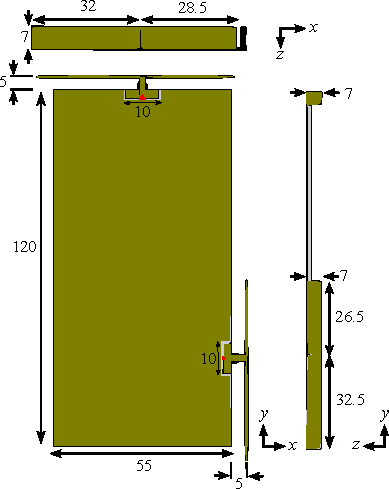
\includegraphics[scale=0.7]{img/Lasse/3d_drawing_mini.pdf}
    \end{center}
  \end{columns}
\end{frame}

\begin{frame}
  \frametitle{Ground Clearance}
    \begin{center}
      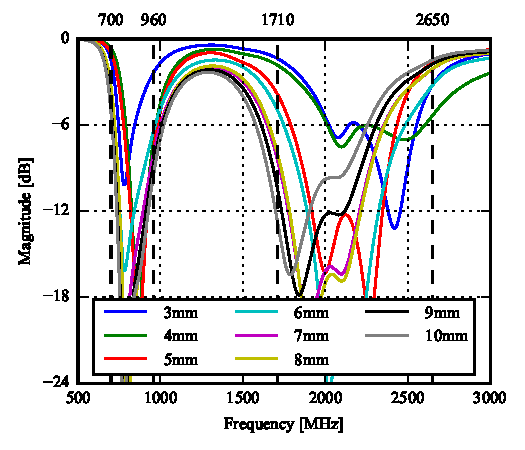
\includegraphics[scale=0.7]{img/Lasse/s11_5mm.pdf}
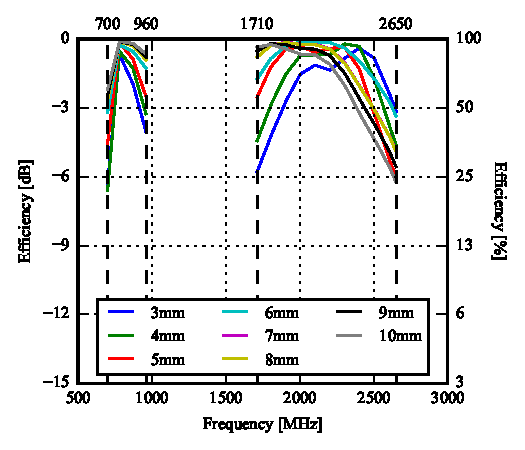
\includegraphics[scale=0.7]{img/Lasse/eff_5mm.pdf}
    \end{center}
      \begin{itemize}
      \item Significant bandwidth and efficiency drop from \SI{5}{mm} to \SI{4}{mm}.
      \end{itemize}
\end{frame}

\section[Tuner PCB]{Tuner PCB (Lasse)}
\begin{frame}[fragile]
    \frametitle{Tuner PCB with MEMS Tuner}
\begin{center}
            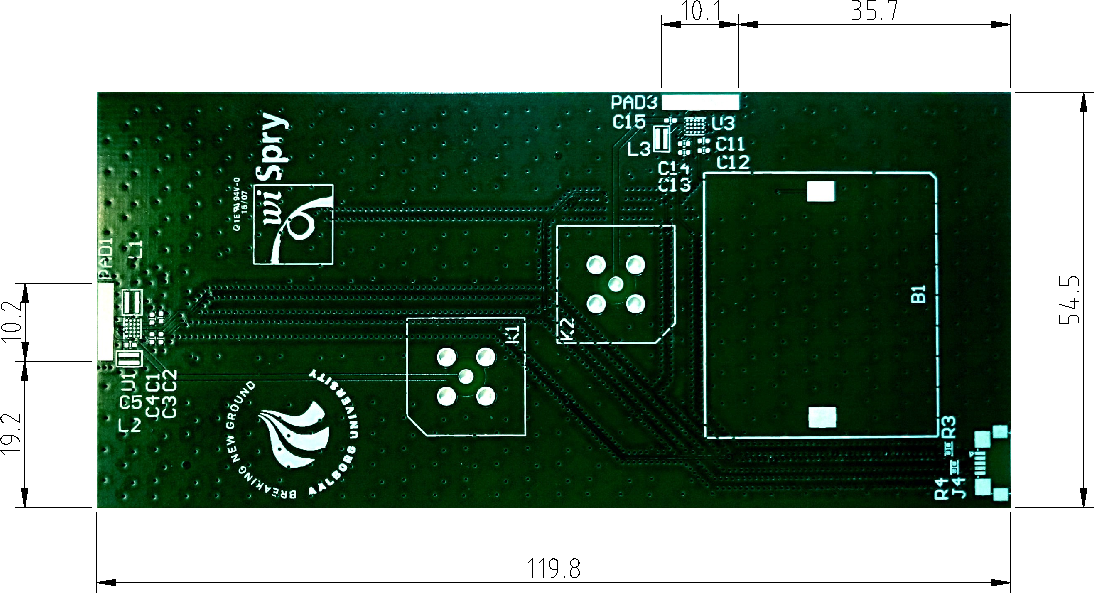
\includegraphics[scale=0.5]{img/Lasse/samanthas_board.pdf}
\end{center}
\begin{itemize}
\item Use previously made Tuner PCB -- save time.
\end{itemize}
\end{frame}

\begin{frame}
  \frametitle{Tuner PCB Results}
  \begin{itemize}
  \item Problems with detuning in the high frequencies.
  \end{itemize}
  \begin{center}
    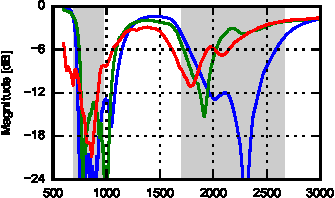
\includegraphics{img/Lasse/tuner_pcb/001_s11top.pdf}
    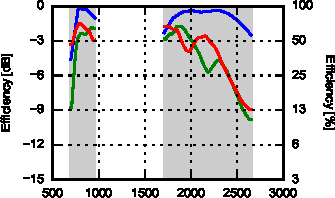
\includegraphics{img/Lasse/tuner_pcb/001_efftop.pdf} \\
    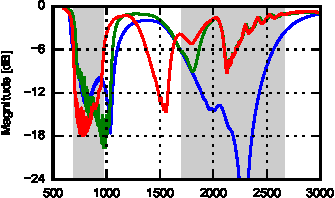
\includegraphics{img/Lasse/tuner_pcb/001_s22side.pdf}
    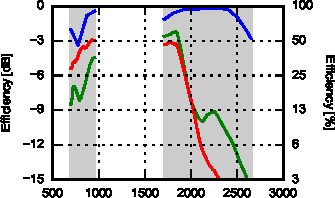
\includegraphics{img/Lasse/tuner_pcb/001_effside.pdf}
  \end{center}
\legendfooter
\end{frame}

\begin{frame}[fragile]
    \frametitle{Tuner PCB -- Modified Design}
    \begin{columns}[onlytextwidth,t]
        \column{0.49\linewidth}
          \begin{itemize}
          \item Adding of a higher resonant to counteract the detuning.
          \item Two arms added in the available space. 
          \item Ground clearance \SI{2.5}{mm}.
          \end{itemize}
        \column{0.49\linewidth}
        \begin{center}
            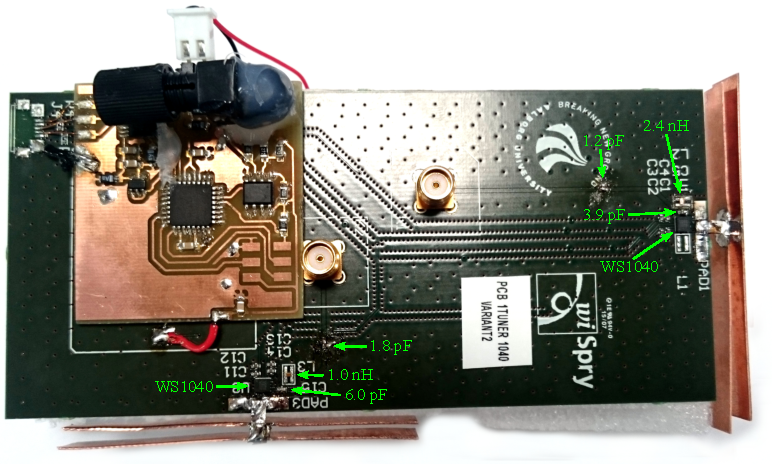
\includegraphics[scale=0.33, angle =90]{img/Lasse/lassedouble.pdf}
            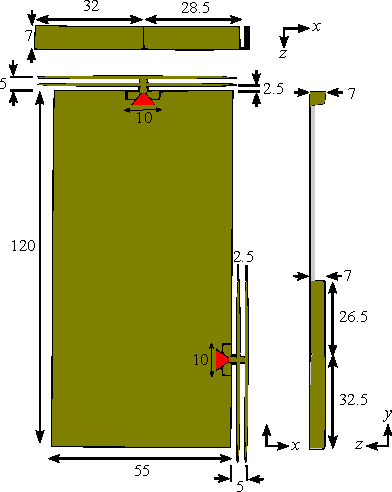
\includegraphics[scale=0.53]{img/Lasse/3d_drawing_modi.pdf}
        \end{center}
        Tuner PCB with the modified monopole.
    \end{columns}
\end{frame}
\def\legendfooter{\scriptsize{Upper: Top antenna. Lower: Side antenna. \textcolor{bb}{Monopole Sim}, \textcolor{gg}{Monopole Meas}, Frequency in MHz.}}
\def\emptyline{\textcolor{white}{Empty}}

\begin{frame}
  \frametitle{Modified Monopole Results.}
\begin{center}
    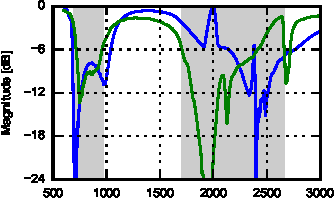
\includegraphics{img/Lasse/tuner_pcb/002_s11top.pdf}
    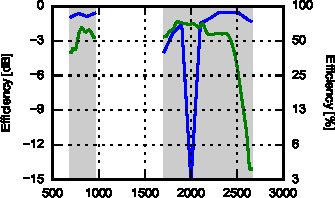
\includegraphics{img/Lasse/tuner_pcb/002_efftop.pdf} \\
    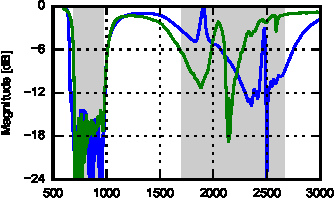
\includegraphics{img/Lasse/tuner_pcb/002_s22side.pdf}
    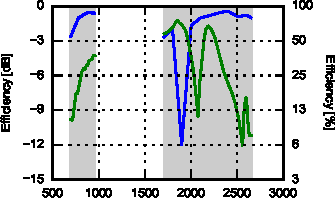
\includegraphics{img/Lasse/tuner_pcb/002_effside.pdf}
\end{center}
      \begin{itemize}
      \item Shunt capacitor on transmission lines.
      \end{itemize}
\legendfooter
\end{frame}
\def\legendfooter{\scriptsize{Upper: Top antenna. Lower: Side antenna. \textcolor{bb}{Monopole without cap}, \textcolor{gg}{Monopole with cap}, Frequency in MHz.}}
\def\emptyline{\textcolor{white}{Empty}}

\begin{frame}
  \frametitle{Tuner PCB}
  \begin{itemize}
  \item With and without transmission line shunt capacitor.
  \item Straight forward ``finger sweep''.
  \end{itemize}
\begin{center}
    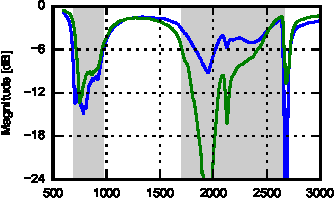
\includegraphics[scale=1.4]{img/Lasse/tuner_pcb/003_s11top.pdf}
\end{center}
\begin{itemize}
\item Increase in bandwidth in the high band.
\item Most significant for S11 but is also the case for S22 
\end{itemize}
\legendfooter
\end{frame}

\section[Conclusion]{Conclusion (Lasse)}
\begin{frame}
  \frametitle{Conclusion}
  \begin{block}{Sub-subject 1}
    \begin{itemize}
    \item Three preliminary designs.
    \item Two designs on the tuner PCB.
    \item Modified \SI{2.5}{mm} ground clearance design.
    \item Promising prototype results comparable with state-of-the-art designs.
    \item Problems with the resonance in the higher frequencies.
    \item MIMO support in the high band -- high correlation in the low band.
    \end{itemize}
  \end{block}
  \begin{block}{Sub-subject 2}
    \begin{itemize}
    \item Simulation of Tuner PCB.
    \item New Tuner PCB.
    \item Modified monopole not necessary. 
    \item Different \SI{5}{mm} antenna designs.
    \item Two different designs on the PCB.
    \end{itemize}
  \end{block}
\end{frame}
